\section{Introduction}
\label{sec:intro}
Predicting ``what happens next'' in narrative stories is an important
but challenging task called commonsense reasoning in artificial intelligence.
Story comprehension was first studied in the context of 
planning and goal searching~\cite{meehan1977tale}, which was one of the
most important problems in AI. The task and evolved with
the work of Chambers and Jurafsky~\shortcite{chambers2008unsupervised}
which attracts more attention on predicting what is expected to happen next in stories.
Later, \scite{mostafazadeh2016corpus} release a standard dataset called
SCT (Story Cloze Test) for the evaluation of this task.
SCT requires a system to choose the correct ending of a four-sentence
story context from two alternatives.
\figref {fig:story} shows an story example which
contains four context sentences and two candidate endings.


\begin{figure}[th]
\centering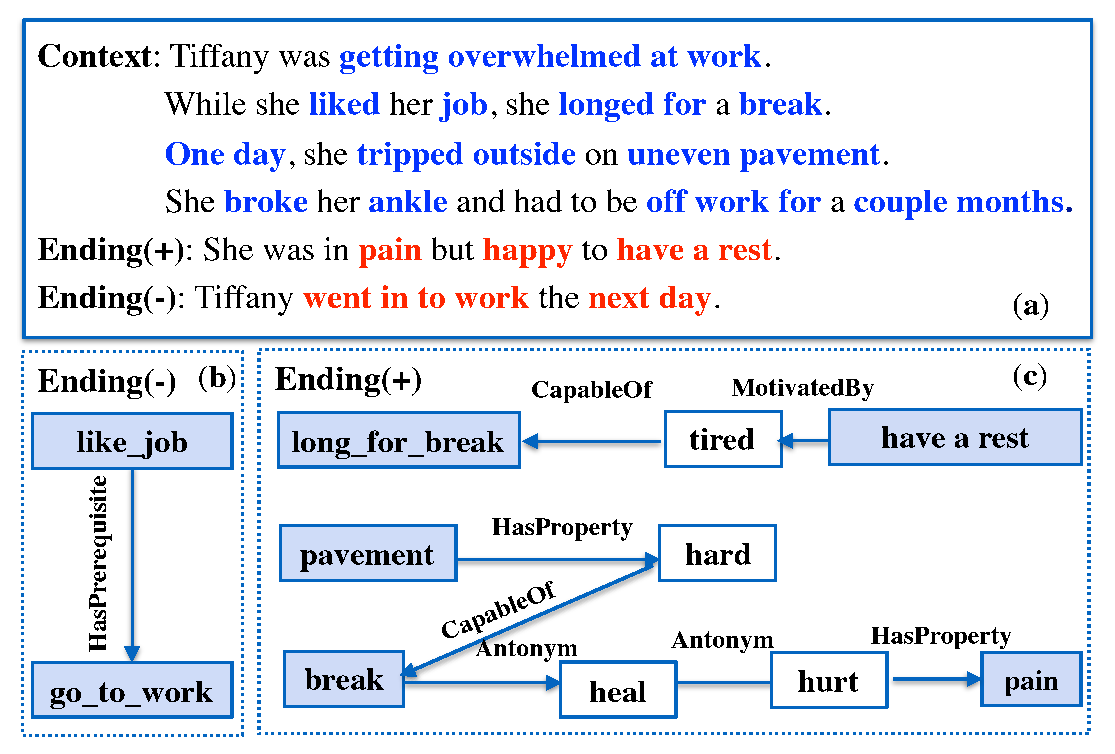
\includegraphics[width=3.5in]{pictures/story_example}
\caption{Example from the story-cloze task: given a short story, predict the correct ending from two choices. In (b) and (c), the words in the blue boxes are concepts from the story; the words in the white boxes are concepts not from the story but serve as bridging nodes.}
\label{fig:story}
\end{figure}

%\begin{figure}[th]
%\small
%\begin{tabular}{ll} \hline
%\\
%Context: & Tiffany was \textcolor{blue}{getting overwhelmed at work}. \\
 %& While she \textcolor{blue}{liked} her \textcolor{blue}{job} she \textcolor{blue}{longed for} a \textcolor{blue}{break}. \\
 %& One day, she \textcolor{blue}{tripped outside} on uneven pavement. \\
 %& She \textcolor{blue}{broke} her \textcolor{blue}{ankle} and had to be \textcolor{blue}{off work} for \\
 %& a couple of months. \\
%Ending(+): & She was \textcolor{blue}{in pain} but \textcolor{blue}{happy} to \textcolor{blue}{not} have to \textcolor{blue}{go to work}. \\
%Ending(-): & She \textcolor{blue}{went in to work} the next day \\
%\\
 %\hline
%\end{tabular}
%\centering\includegraphics[width=3.5in]{pictures/story}
%\caption{Example from the story-cloze task: predict the correct ending to a given short story out of provided options.}\label{fig:story}
%\end{figure}

Most early studies treat this task as a supervised binary classification problem.
However, this was not the original intention
of \scite{mostafazadeh2016corpus} who proposed the SCT dataset, 
because the training data has approximately 100,000 five-sentence stories,
without providing any negative endings.
%because the dataset didn't provide any
%binary classification training data, but only approximately 100,000
%five-sentence stories without negative endings.
To overcome the lack of training set, many researchers train their classifier using
the smaller validation set from SCT, 
which consists of 1,871 stories with annotated positive and negative endings.
%the smaller validation set from SCT, which consists of both positive and
In our study (\secref{sec:dataset}), we find there is significant bias in
the positive and negative endings of the stories provided in the validation
set, which causes information leak.
We argue that it is unreliable and also expensive to manually create and
label negative endings for stories,
and that validation set is not suitable for training
or even fine-tuning the predicting models.
%In addition, training with only about 1500 validation stories is contrary to ~\citeauthor{mostafazadeh2016corpus} 's original intention that actually understanding the underlying narrative from large quantity of narrative knowledge.
Instead, we propose to define the SCT story ending predicting task as a
semi-supervised learning problem. We train the prediction classifier on
the training set (with only positive endings),
as well as automatically generated negative endings.

Previous researches on this topic generally follow a two-step representation:
first represent the individual sentence with shallow linguistic features,
and then aggregate the sentence representations into a story context
representation~\cite{mostafazadeh2016story,li2018multi,chen2018incorporating,zhou2019story}.
Because most of these approaches use complex neural models
with large number of parameters,
they require large amount of training data.
Unfortunately, stories for training come in limited quantity,
and contain much variance and noises, distracting most of these models.
Moreover, most of these methods did not properly model the
commonsense relations between the sentences when aggregating
the sentence representations.

%The first two genres represent the story from different perspectives.
%Many feature-based models represent a whole story with the external shallow
%linguistic features such as word embedding, character features,
%part-of-speech (POS) taggings, sentiment polarity of a word and
%negation~\cite{li2018multi}. However, these methods ignore the semantic
%structure in the story line, which is important for story understanding.
%The neural models represent each sentence with low-dimensional dense
%vectors~\cite{mostafazadeh2016story}.
%The sentence vectors are trained with different language models from
%a larger corpus, such as the BookCorpus, which contains 11,000 books.
%However, without sufficiently enough training resources, it is hard to
%learn the reasoning logic and an efficient representation.
%The third line incorporates the language features in neural model.
%For example, \citeauthor{chen2018incorporating} and ~\citeauthor{zhou2019story} apply
%ConceptNet~\cite{speer2017conceptnet}, a commonsence knowledge base,
%to extract the commonsense features between any two sentences in
%a story.

In this paper, we are committed to improving the story representation
using commonsense knowledge following the same two-step approach.
Two key ideas are listed below.

First, we simplify each sentence by extracting a sequence of
ConceptNet~\cite{speer2017conceptnet} concepts from the sentence
and obtain the {\em intra-sentence} concept representation.
By simplifying the sentences, we are essentially reducing the noise
and variance in the training data, which allows a better model to
be trained given limited amount of data.
In \figref{fig:story}, each colored phrase (multi-word expression)
matches a concept from ConceptNet,
whereas other words are not important for understanding
the story. Therefore we keep only the colored words
from each sentence to represent the main idea of the story.
Then we use a sequential language model, inspired by
Skip-thought~\cite{kiros2015skip} obtaining the
semantic representation of each simplified sentence.

Second, we take in the structured commonsense knowledge of concepts from ConceptNet.
In ConceptNet, there exist paths between key concepts in the story.
For example, ``long for break'' is related to ``have a rest''
through {\em CapableOf} and {\em MotivatedBy} relation edges.
These edges help us ``connect the dots'' within the story and allows us
to make more meaningful deduction through the story line.

In summary, this paper makes the following contributions:
\begin{itemize}
\item We simplify the stories by streamlining sentences to a few
key concepts, which eliminates unwanted variance in the text,
and makes training easier and more reliable;
(\secref{sec:sentence simplification})
\item We combine sequential and structured representation for the key concepts
in a sentence as the sentence representation.
This kind of representation takes into account the inter-sentence semantics
and the external structured commonsense knowledge; (\secref{sec:represent})
\item Experimental results show that our sentence representation in story
significantly improves the accuracy of story ending prediction. (\secref{sec:result})
\end{itemize}
